% !TEX root = main.tex
% !TEX program = pdflatex


\section{Especificação e montagem do protótipo}
\label{sec:montagem}

Conforme mencionado nas seções anteriores, o robô construído possui três rodas em uma configuração simétrica. Apesar da falta de redundância -- pois se alguma das rodas falhar se perde a holonomicidade --, robôs omnidirecionais com 3 rodas (TOMR) são utilizados com mais frequência por serem mais simples de se implementar, apresentarem custo mais baixo (pois motores e rodas são responsáveis por 53\% do custo do projeto, conforme o \hyperref[sec:custo]{Apêndice A}), e uma certa economia de peso. As rodas utilizadas -- mostradas na Figura \ref{fig:omniwheel} --, medem 58 mm de diâmetro, com estrutura em plástico e dez roletes emborrachados, e possuem capacidade de carga nominal de 3 kg \citep{omniwheel}, suficiente para os fins de demonstração do projeto. Cada roda é acionada por um motor de corrente contínua com caixa de redução, com uma velocidade nominal no eixo de saída de 210 rpm para uma tensão de 6 V. A máxima potência do motor está especificada para uma corrente de 1,1 A, a 110 rpm. Incluso no motor está um \textit{encoder} de quadratura, que permite a leitura da velocidade da roda e da direção de rotação. Com a relação de redução, se tem que para cada revolução da roda se tem 341,2 pulsos do sensor, e portanto cada pulso representa 0.01841 radianos \citep{motor}.
%Mais info sobre a ponte H: http://linksprite.com/wiki/index.php5?title=DC_Motor_Driver_Breakout_%28L298_Chipset%29#Arduino_Sample_Code

Além da utilização dos \textit{encoders} para implementação da odometria, também foi instalada na estrutura uma bússola, para garantir uma medida absoluta da orientação do robô (sem os erros que se acumulam nos métodos de \textit{dead-reckoning}). O modelo utilizado é a HMC5883L, já instalada em uma placa com alguns componentes necessários para seu funcionamento. A precisão do circuito, de acordo com o fabricante, é de 2 graus \citep{HMC5883L}. Para complementar a odometria, também foi instalada no robô uma unidade de medidas inerciais MPU6050, que possui acelerômetro e giroscópio em torno dos três eixos utilizados \citep{MPU6050}. Os sensores descritos neste parágrafo foram adquiridos e montados à estrutura, porém não foi realizada sua implementação. Os dois periféricos utilizam o protocolo de comunicação I2C \citep{semiconductors2000i2c}, também compatível com o computador utilizado.

Foi adquirida também uma bateria NiCd, com capacidade de carga de 2000 mAh e 7,2 V de tensão nominal. Este tipo de bateria se caracteriza por apresentar recarga rápida e boa capacidade de utilização com correntes altas. Ligados à bateria, se tem 2 reguladores de tensão \textit{step down} MP2307, especificados para fornecer corrente constante de até 3 A cada um, suportando picos de até 4 A \citep{MP2307}. A tensão de saída dos reguladores foi configurada em 5.1 V (para o computador) e 6 V (para os motores). Como cada motor opera em geral com correntes abaixo de 1 A, o regulador utilizado é adequado, porém apresenta margens de capacidade consideravelmente pequenas. Os \textit{encoders} sãp alimentados pelo próprio computador, que possui saída regulada de 3,3 V capaz de fornecer até 500 mA \citep{upton2014raspberry}. A bússola e a IMU tem tensão de alimentação de 3,3 V, podendo ser adicionado ao sistema mais um regulador de tensão quando forem eventualmente integradas ao sistema, pois há espaço suficiente no chassi para tal. Neste caso, se recomenda alimentar os \textit{encoders} a partir do mesmo regulador.

O acionamento dos motores se dá por um circuito de pontes H. Há duas destas placas, e cada uma pode acionar dois motores. Assim, se tem a possibilidade de utilizar mais um motor (ou outro atuador) em trabalhos futuros. Os \textit{drivers} são desenvolvidos em torno do circuito L298N, que pode fornecer 4 A de corrente contínua distribuída entre as cargas \citep{L298N}. O chaveamento de cada canal dos \textit{drivers} é feito por meio de modulação de largura de pulso, fornecida pelo computador. Assim como os demais componentes, os \textit{drivers} foram fornecidos integrados a uma placa montada, com terminais para fixação de cabeamento e dissipadores de calor.

Todo o processamento é realizado por um \textbf{Raspberry Pi}, um \emph{single board computer}, que utiliza a arquitetura \acrshort{arm} em seu processador, ideal para dispositivos alimentados por baterias por consumir pouca energia e gerar pouco calor. O processador possui quatro núcleos, e um \emph{clock} de 1,2 GHz -- poder computacional equivalente há um computador de mesa comum. O \acrshort{rpi} utiliza um sistema operacional GNU/Linux, e \emph{software} deve ser desenvolvido para ser executado nesta plataforma. Há ainda 40 pinos de \acrshort{gpio} que podem ser utilizados para conectar sensores, atuadores e diversos componentes, e suporte nativo a \acrshort{i2c} \citep{upton2014raspberry}.

Para unir todos os componentes descritos, se projetou uma estrutura central, como um chassi. Tal estrutura pode ser vista na Figura \ref{fig:chassi}. No centro geométrico da estrutura e na periferia, próximo a uma das rodas, foram feitos dois orifícios que devem acomodar uma caneta hidrográfica cada. Assim, durante a fase de testes, se pode acompanhar graficamente a evolução cinemática do robô. Devido a localização central de uma das canetas, todos os componentes foram instalados na periferia da estrutura. Se tomou ainda o cuidado de instalar os CI de acelerômetro e giroscópio o mais próximo ao centro possível, para que as componentes de aceleração centrípeta dos movimentos com componentes de rotação não influenciassem em demasiado nos resultados. A IMU poderia ter sido colocada no centro geométrico, e este erro poderia ser introduzido no traço da caneta. No entanto, como a odometria e localização dependem muito mais dos sensores montados nos motores do que da IMU, se preferiu manter a caneta no centro, mantendo o MPU6050 o mais próximo possível. A bússola também foi montada relativamente próxima ao centro do robô, se tomando o cuidado de alinhar os eixos dos sistemas de coordenadas dos sensores com os do robô.

\begin{figure}[h]
  \centering
  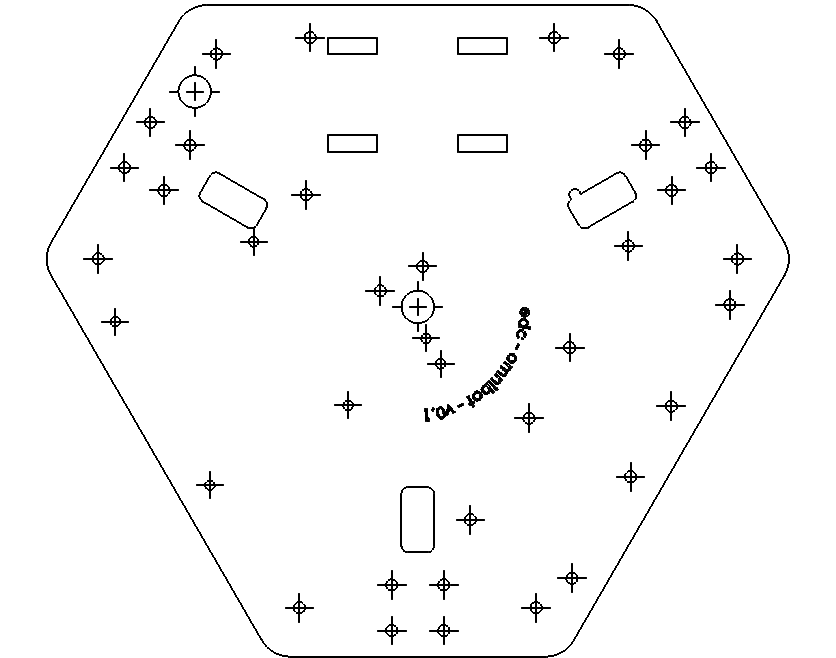
\includegraphics[width = 0.45\textwidth]{imagens/chassidxf}
  \caption{Chassi projetado.}
  \label{fig:chassi}
\end{figure}

Todos os componentes adquiridos possuem furos para fixação por meio de parafusos com 3 mm de diâmetro. A estrutura foi projetada com furos de 3,5 mm de diâmetro, para compensar possíveis erros de medição (visto que nem todos os componentes apresentaram seus desenhos nas informações técnicas) e possíveis tolerâncias de fabricação. Além dos furos de fixação dos componentes, também foram introduzidos orifícios próximos aos motores, para passagem dos cabos de um lado a outro da placa, e orifícios para fixação da bateria com presilhas plásticas. Na mesma área destinada à fixação da bateria se adicionou furação capaz de receber uma placa Arduino MEGA, caso se deseje utilizar um microcontrolador em trabalhos futuros. Também foram adicionados 6 furos na periferia do chassi, para possibilitar a montagem de outra chapa sobre a dos componentes, caso sejam realizados trabalhos que exijam a expansão da estrutura.

A plataforma projetada foi então fabricada, utilizando chapas de acrílico transparente de 5 mm de espessura. Se cogitou produzir tal estrutura em alumínio, porém se mostrou mais prático utilizar o acrílico. Entre as vantagens do material plástico se podem destacar a fácil obtenção, baixo custo, isolamento elétrico (permitindo montar os componentes eletrônicos diretamente sobre o chassi) e a possibilidade de fabricação utilizando uma máquina de corte a \textit{laser}, que elimina o limite inferior de tamanho de brocas e fresas em relação a fresadora CNC considerada originalmente. A espessura foi escolhida empiricamente, dentro das disponíveis, de maneira relativamente conservadora, e atendeu as necessidades. Na Figura \ref{fig:montagem} se pode ver a montagem final do protótipo. Os furos sobredimensionados não afetaram o alinhamento das peças.

\begin{figure}[h]
  \centering
  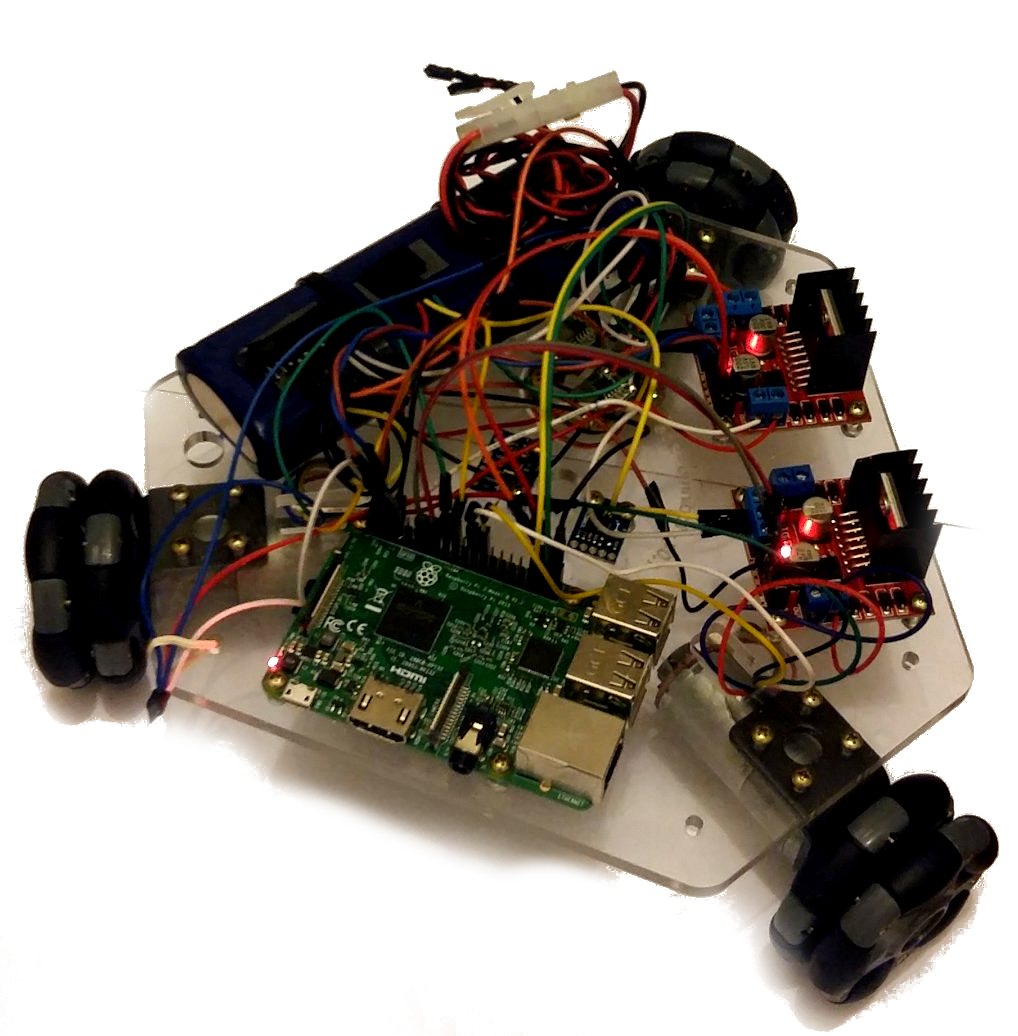
\includegraphics[width = 0.45\textwidth]{imagens/roboto}
  \caption{Protótipo montado, sem as canetas.}
  \label{fig:montagem}
\end{figure}

A bateria foi fixada sobre a estrutura utilizando presilhas plásticas. Ao redor da bateria foram fixados 3 barramentos, para aterramento, alimentação dos \textit{drivers} e alimentação dos \textit{encoders}. Foram instalados um conector para a bateria e outro conector para o caso em que se deseja utilizar uma fonte externa.  Além dos fios que alimentam os reguladores de tensão, um par de fios sobressalente (conectados ao terminal positivo e negativo da fonte ou bateira) foi instalado junto a estes conectores, e pode ser utilizado em trabalhos futuros.

O custo de aquisição dos componentes relatados pode ser visto detalhado no \hyperref[sec:custo]{Apêndice A}. Cabe ressaltar que todos os itens foram comprados em dobro, para realizar a montagem de dois robôs para futuros trabalhos no LAMECC (Laboratório de Mecatrônia e Controle). Mais detalhes sobre as dimensões do chassi podem ser vistos no diagrama apresentado no \hyperref[sec:draw]{Apêndice C}.

\section{Desenvolvimento Teórico}
\label{sec:teorico}

%% MODELAGEM:
%PARK: pg 468
\subsection{Modelagem Cinemática}

Primeiramente, se definem dois sistemas de coordenadas. O primeiro, $(x_I,y_I)$, é o sistema de coordenadas global, fixo no ambiente. O segundo, $(x_R,y_R)$, está centrado no próprio robô. Ainda se pode definir o ângulo $\theta$ como a orientação do robô -- ou seja, o ângulo entre os dois sistemas de coordenadas. Tal relação pode ser vista na Figura \ref{fig:ref}, e a transformação de um sistema para o outro é descrita na Equação \ref{eq:world_ref}, conforme \citet{siegwart2011introduction} e \citet{ritter2016modelagem}.

\begin{figure}[h]
  \centering
  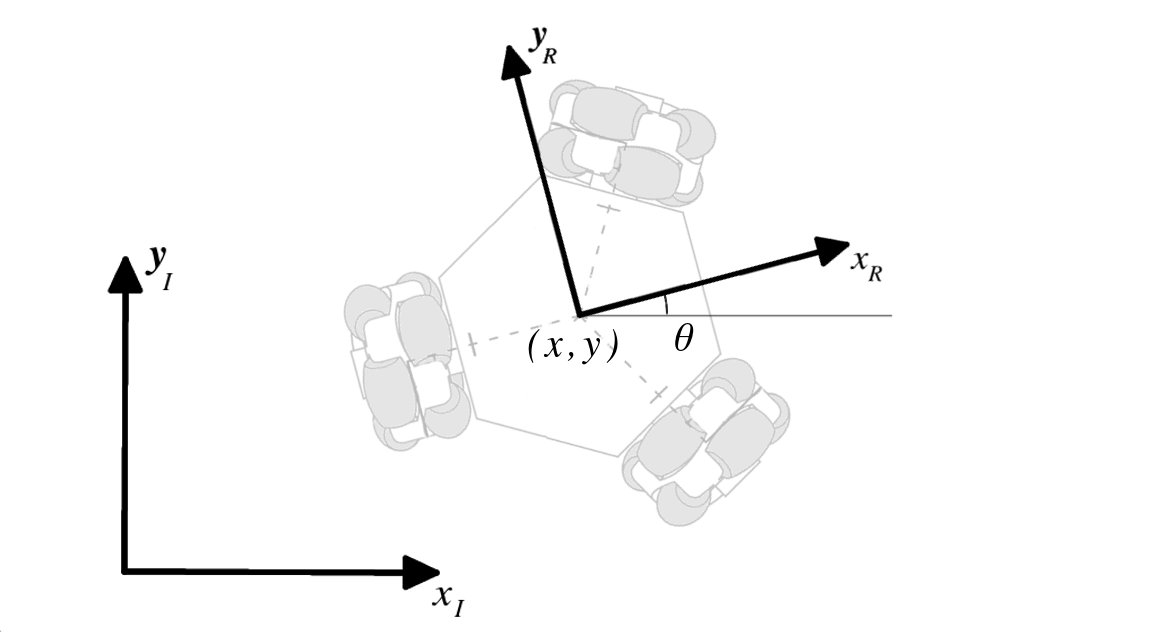
\includegraphics[width = 0.65\textwidth]{imagens/ref}
  \caption{Sistemas de coordenadas global I e relativo ao centro do robô R.}
  \source{Adaptado de \citet{ritter2016modelagem}}
  \label{fig:ref}
\end{figure}

\begin{equation}
  \begin{pmatrix}
    x_I \\
    y_I \\
    \theta
  \end{pmatrix}
  =
  \begin{pmatrix}
    cos \theta & -sen \theta & 0 \\
    sen\theta  &  cos \theta & 0 \\
    0          & 0          & 1
  \end{pmatrix}
  \begin{pmatrix}
    x_R \\
    y_R \\
    \theta
  \end{pmatrix}
  \label{eq:world_ref}
\end{equation}

O último termo da Equação \ref{eq:world_ref} também pode ser descrito como $q_R$, e o vetor de velocidades $[v_x, v_y, \omega_z]^T$, centrados no sistema de coordenadas do robô, é $\dot{q_R}$. Com o objetivo de mapear a velocidade de giro das rodas $\dot{\phi} = [\dot{\phi}_1, \dot{\phi}_2, \dot{\phi}_3]^T$ às velocidades $\dot{q_R}$, se utiliza a modelagem cinemática apresentada por \citet{siegwart2011introduction}, com as referências apresentadas na Figura \ref{fig:robo_vel}. Na figura,  A mesma modelagem é utilizada por \citet{ritter2016modelagem}, porém com outra sequência e sentido de giro para as rodas.

\begin{figure}[h]
  \centering
  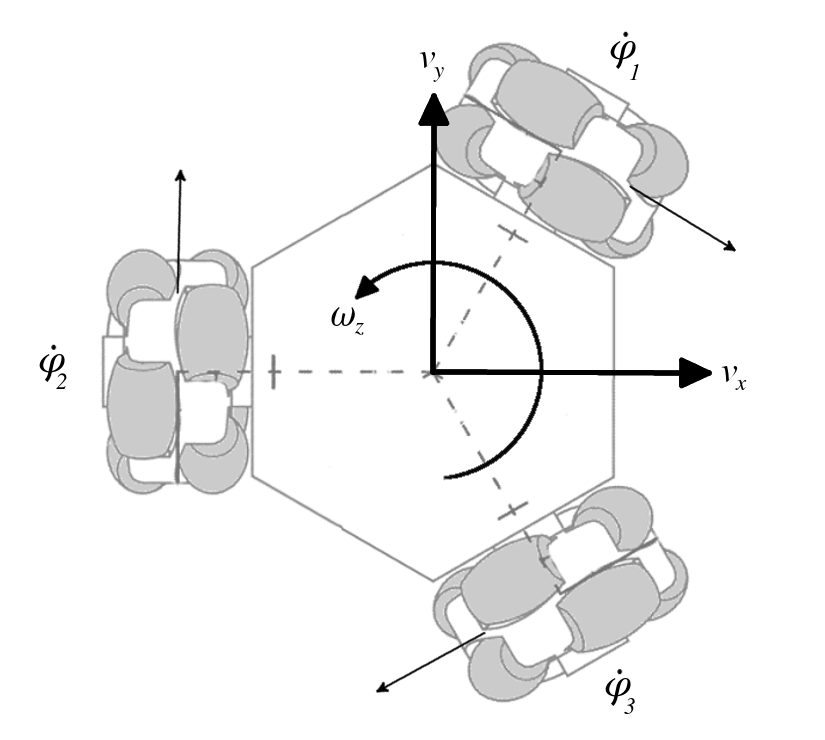
\includegraphics[width = 0.5\textwidth]{imagens/robot_vel4}
  \caption{Vista superior do robô, mostrando as convenções adotadas. As grandezas $v_x$ e $v_y$ estão no sistema de coordenadas do robô.}
  \label{fig:robo_vel}
\end{figure}

Assim, para um robô com 3 rodas dispostas em simetria radial em torno do centro da estrutura, a cinemática direta é dada pela Equação \ref{eq:dk}. Diversos autores utilizam variações da mesma modelagem (\citet{rojas2006holonomic}, \citet{pin1994new}, entre outros). Nas equações apresentadas, $r$ é o raio de cada roda e $R$ o raio do robô (a distância do centro da roda ao centro da estrutura do robô).

\begin{equation}
  \begin{pmatrix}
    v_x \\
    v_y \\
    \omega_z
  \end{pmatrix}
  =
  \frac{r}{3R}
  \begin{pmatrix}
    -\frac{3R}{\sqrt{3}} & 0   & \frac{3R}{\sqrt{3}} \\
    R                    & -2R & R                   \\
    1                    & 1   & 1
  \end{pmatrix}
  \begin{pmatrix}
    \dot{\phi_1} \\
    \dot{\phi_2} \\
    \dot{\phi_3}
  \end{pmatrix}.
  \label{eq:dk}
\end{equation}

Também se deseja utilizar a cinemática inversa do modelo, obtida realizando-se a inversão da matriz de transformação apresentada na Equação \ref{eq:dk}, é dada pela Equação \ref{eq:ik}. Nota-se que esta inversão é simplificada no caso do robô com 3 rodas, visto que quando há mais rodas é formada uma matriz $3 \times n$, sendo $n$ o número de rodas, e se deve utilizar uma matriz pseudo-inversa, conforme demonstrado por \citet{rojas2006holonomic}.

\begin{equation}
  \begin{pmatrix}
    \dot{\phi_1} \\
    \dot{\phi_2} \\
    \dot{\phi_3}
  \end{pmatrix}
  =
  \frac{1}{r}
  \begin{pmatrix}
    -\frac{\sqrt{3}}{2} & \frac{1}{2} & R \\
    0                   & -1          & R \\
    \frac{\sqrt{3}}{2}  & \frac{1}{2} & R
  \end{pmatrix}
  \begin{pmatrix}
    v_x \\
    v_y \\
    \omega_z
  \end{pmatrix}
  \label{eq:ik}
\end{equation}

Como pela classificação de \citet{campion1996structural} um \acrshort{tomr} é caracterizado na categoria (3,0), o modelo cinemático das equações \ref{eq:dk} e \ref{eq:ik} é controlável, estável e descreve a posição, orientação e suas derivadas de forma suficiente. % O modelo cinemático da Equação \ref{eq:dk} também é utilizado por \citet{rojas2006holonomic} e \citet{ritter2016modelagem}.

%% ODOMETRIA:
% lynch, pg 492 do pdf
\subsection{Odometria}

Durante a operação do robô, se torna necessário calcular a posição da estrutura. Para o cálculo da odometria, se utiliza a metodologia mostrada em \citet{lynch2017modern}. Se assume que durante um certo intervalo de tempo $\Delta t$ se tenha velocidades de rotação constantes nas rodas, o que permite considerar $\dot{\phi_i}.\Delta t = \Delta \phi_i$. Considera-se também que a unidade de tempo deste período é arbitrária, e como se deseja integrar no mesmo intervalo posteriormente, se assume um período unitário $\Delta t = 1$. Este procedimento está descrito na Equação \ref{eq:odo}, modificada a partir da Equação \ref{eq:dk}. Na prática, é fácil contar os deslocamentos angulares $\Delta \phi_i$, visto que o número de pulsos por revolução dos \textit{encoders} é determinado.

\begin{equation}
  \begin{pmatrix}
    v_x \\
    v_y \\
    \omega_z
  \end{pmatrix}
  =
  \frac{r}{3R}
  \begin{pmatrix}
    -\frac{3R}{\sqrt{3}} & 0   & \frac{3R}{\sqrt{3}} \\
    R                    & -2R & R                   \\
    1                    & 1   & 1
  \end{pmatrix}
  \begin{pmatrix}
    \Delta{\phi_1} \\
    \Delta{\phi_2} \\
    \Delta{\phi_3}
  \end{pmatrix}.
  \label{eq:odo}
\end{equation}

De posse das velocidades da plataforma durante o período de tempo unitário $\Delta t$ -- lembrando que $v_x$, $v_y$ e $\omega_z$ estão no sistema de coordenadas centrado no corpo do robô --, se deve avaliar o deslocamento em relação ao centro do robô na posição anterior. Para o caso em que $\omega_z = 0$, numa trajetória retilínea, se tem simplesmente que $\Delta q_R = \dot{q_R}$.

No entanto, quando houve mudança de orientação no período e consequentemente $\omega_z \neq 0$, se deve levar em consideração os desvios de trajetória causados por essa rotação. Assim, se obtem $\Delta q_R$ de acordo com a Equação \ref{eq:desvio} \citep{lynch2017modern}.

\begin{equation}
  \Delta q_R
  =
  \begin{pmatrix}
    \Delta x_R \\
    \Delta y_R \\
    \Delta\theta
  \end{pmatrix}
  =
  \begin{pmatrix}
    (v_x sen(\omega_z)) + v_y (cos(\omega_z) - 1)/\omega_z \\
    (v_y sen(\omega_z)) + v_x (1-cos(\omega_z)) / \omega_z \\
    \omega_z
  \end{pmatrix}
  \label{eq:desvio}
\end{equation}

Sendo $k$ o instante antes do período de tempo analisado, para se obter a nova posição $q_I$ do robô no sistema de coordenadas global se deve utilizar a rotação $R(\theta_k)$ apresentada na Equação \ref{eq:world_ref}, e atualizando os valores da última iteração conforme a Equação \ref{eq:new_odo}.

\begin{equation}
  q_{I(k+1)} = q_{I(k)} + \Delta q_I = q_{I(k)} + R(\theta_k) \Delta q_I
  \label{eq:new_odo}
\end{equation}
%\cite{samani2007comprehensive}: Adicionam um modelo de ruído dos encoders à estimativa. TIRAR OU ELABORAR?

%% PLANEJAMENTO DE TRAJETÓRIA:
\subsection{Planejamento de Trajetória}

Para o robô desenvolvido, não há a necessidade de implementar algoritmos complexos de planejamento de trajetória (detecção de obstáculos, caminhos de mínima energia, etc.). Serão abordados caminhos ``ponto a ponto'', que levam de um ponto inicial a um ponto final, ambos em repouso \citep{lynch2017modern}.

Apesar de ser uma trajetória simples, ainda se podem aplicar considerações para uma melhor operação do sistema. Uma dessas considerações é o chamado \textit{time-scaling} da trajetóra, ou seja, a geração de uma função $s(t)$ que suavize o comportamento do robô por meio de restrições em velocidades e acelerações. Na Figura \ref{fig:poly5} se pode ver uma curva de perfil de velocidade polinomial de quinta ordem, que pode garantir velocidades e acelerações nulas nos pontos de origem e destino.

\begin{figure}[h]
  \centering
  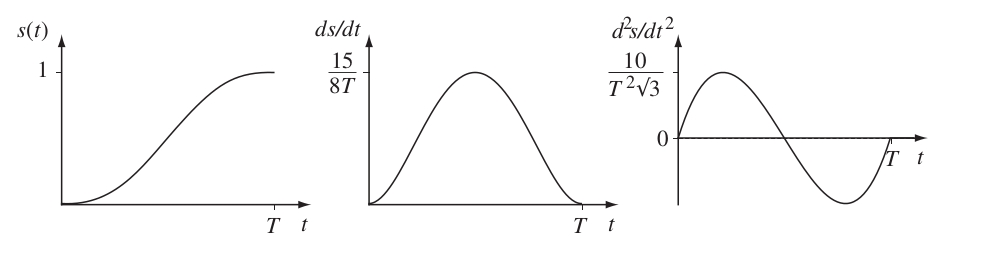
\includegraphics[width = 0.85\textwidth]{imagens/poly5}
  \caption{Deslocamento, velocidade e aceleração durante uma trajetória gerada por polinômio de quinta ordem. Aceleração e velocidade são nulas tanto no ponto de origem quanto no ponto de destino.}
  \source{\citet{lynch2017modern}}
  \label{fig:poly5}
\end{figure}

No entanto, a interpolação de um polinômio a cada cálculo de trajetória é um processo que pode envolver um certo custo computacional elevado, e devido à simplicidade dos componentes utilizados, se julgou que o aumento de suavidade na operação não fosse significativo. Portanto, neste trabalho se optou por utilizar um perfil de velocidade trapezoidal, conforme mostrado na Figura \ref{fig:trap}. Tal perfil é um dos mais comuns em robótica, devido a sua simples implementação. Os limites de aceleração foram definidos na fase de implantação do \textit{software}, de modo a evitar o deslizamento das rodas utilizadas na superfície de testes.

\begin{figure}[h]
  \centering
  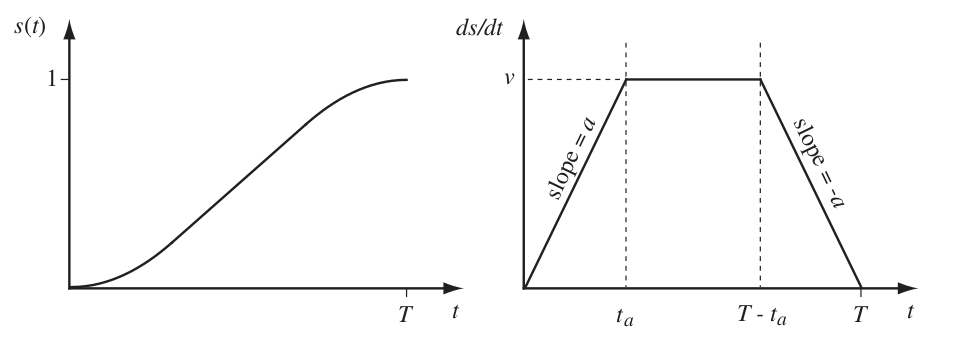
\includegraphics[width = 0.63\textwidth]{imagens/trapezoidal}
  \caption{Deslocamento e velocidade durante um deslocamento com perfil de velocidades trapezoidal. Tal perfil foi adotado neste trabalho.}
  \source{\citet{lynch2017modern}}
  \label{fig:trap}
\end{figure}

Utilizando a curva do perfil de velocidade, se pode fixar setpoints de velocidade para cada ponto.

%% CONTROLE:
\subsection{Controle}

SUBSECTION EM CONSTRUÇÃO

Diversas abordagens podem ser utilizadas para a implantação de controladores em robôs omnidirecionais. Se pode realizar o controle das coordenadas desejadas, em x, y e z, ou o controle da posição de cada roda, independentemente. No caso, foram realizados três controladores de posição, em X, Y e $\omega$, utilizando a odometria discutida acima. O controlador então decide o set point de velocidade para cada roda, e envia os sinais de comando para um conjunto secundário de controladores de velocidade, 1 para cada roda. Se pode ver um esquema do sistema utilzado na FIgura \ref{fig:controle}.

\begin{figure}[h]
  \centering
  
\includegraphics[width = 0.35\textwidth]{imagens/edc}
  \caption{Arquitetura de controle utilizada.}
  %\source{\citet{lynch2017modern}}
  \label{fig:controle}
\end{figure}

Estabilidade, tipo do controle, proporcional, integral, derivativo, digital, tempo de ciclo, q q eu digo aqui, pô?

Não linearidade do tipo zona morta, como será relatado a seguir. COrreção como na Figura \ref{fig:cont_zm}.

\begin{figure}[h]
  \centering
  
\includegraphics[width = 0.35\textwidth]{imagens/edc}
  \caption{Um tipo de correção para não linearidades do tipo zona-morta.}
  %\source{\citet{lynch2017modern}}
  \label{fig:cont_zm}
\end{figure}


\citet{lynch2017modern}:

In most robotic applications, higher control update rates are of limited benefit, given
time constants associated with the dynamics of the robot and environment.

We can use feedforward control, which commands motion even when there
is no error, in combination with feedback control to limit the accumulation of
error:

EQUAÇÃO (11.1) -> EQUAÇÃO (13.11), consigo adaptar pro sinal de controle do motor DC?

This feedforward-feedback controller is the preferred velocity control law.

Loop de velocidade dentro do loop de posição. Posição das rodas ou posição em x e y e $\omega_z$?
Practical Bounds on Feedback Gains According to our simple model,
we could increase K p and K d without bound to make the real components
of the roots more and more negative, achieving arbitrarily fast response. In
practice, however, large gains lead to actuator saturation, rapid torque changes
(chattering), vibrations of the structure due to unmodeled flexibility in the joints
and links, and possibly even instability due to the finite servo rate frequency.
Thus there are practical limits on the set of useful gains.


\citet{rojas2006holonomic}: Sugerem que utilizar um controlador para cada roda é melhor do que para cada grau de liberdade. No nosso caso, é tranquilo pois temos apenas 3 rodas, mantendo o mesmo número de controladores. Devido à realimentação externa lenta, utilizam um preditor no robô. Não entram em detalhes.
motores:
https://www.banggood.com/6V-210RPM-Encoder-Motor-DC-Gear-Motor-with-Mounting-Bracket-and-Wheel-p-1044064.html?p=970719369296201312SG

Given a desired trajectory q d (t), we can adopt the feedforward plus proportional feedback linear controller (11.1) of Chapter 11 to track the trajectory: \cite{lynch2017modern}

\cite{samani2007comprehensive}: Definir os coeficientes dos PIDs é uma novela, pois devemos levar em consideração parâmetros que possuem muita variação, como o coeficiente de atrito do solo, características das baterias, entre outros. Controle deles é bem legal.
%q̇ com (t) = q̇ d (t) + K p ( q̇ d (t) − q(t)),
%(13.11)
%where K p ∈ R 3×3 is positive definite and q(t) is an estimate of the actual con-
%figuration derived from sensors. Then q̇ com (t) can be converted to commanded
%wheel driving velocities u com (t) using Equation (13.7).


%: seguimento de trajetória: malha aberta (3.6.1); Feedback (3.6.2) do livro: It is very similar to the controllers presented in [39, 100]. Others can be found in [8, 52, 53, 137]. Controle com uma matriz de ganhos K para o espaço de estados. Estável e tal. Comentam sobre camadas: planejamento -> decisão -> controlador em tempo real -> hardware.

\subsection{Limitações de Velocidade}

É importante ressaltar que toda a cinemática desenvolvida nas subseções anteriores não considera limites de velocidade para os atuadores. Numa aplicação real, entretanto, existe um ponto de saturação no acionamento de cada motor, que deve ser levada em consideração. Na Figura \ref{fig:twist_sat} se pode ver o efeito dessas limitações, conforme descrito em \citet{lynch2017modern}.

\begin{figure}[h]
  \centering
  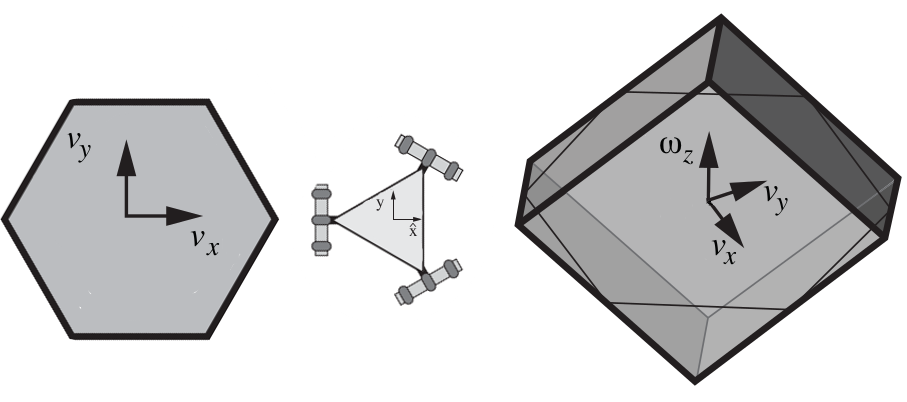
\includegraphics[width = 0.63\textwidth]{imagens/twist_sat}
  \caption{Limites de velocidade translacional e rotacional em função dos limites de saturação dos motores reais.}
  \source{Adaptado de \citet{lynch2017modern} para as coordenadas utilizadas.}
  \label{fig:twist_sat}
\end{figure}

Quando não há rotações ($\omega_z = 0$), o limite de velocidade do corpo do robô é descrito pelo hexágono mostrado na porção esquerda da Figura \ref{fig:twist_sat}: a maior velocidade possível é na direção em que uma das rodas está sendo ``arrastada'', e as componentes de velocidade das outras rodas se somam. Numa situação em que haja necessidade de rotação, a velocidade angular do robô se torna limitada da maneira mostrada no volume tridimensional à direita da Figura \ref{fig:twist_sat}, e se torna fácil enxergar que, para realizar um movimento de rotação na maior velocidade ângular possível, não se pode ter movimentos de translação, para que todos os componentes de velocidade das rodas contribuam apenas para a rotação.

Se pode dizer, então, que para aplicações reais nas quais a holonomicidade da plataforma é de fato desejável, se deve implantar um sistema de planejamento de trajetória que leve em consideração as limitações de velocidade descritas acima.

\section{Implementação dos algoritmos}
\label{sec:software}

Os aspectos teóricos desenvolvidos na seção anterior foram implementados em software para a aplicação prática do sistema. A implementação é, em geral, difícil de se encontrar nos trabalhos da bibliografia, e mesmo que todos os autores descrevessem seus algoritmos em detalhes, os rápidos avanços na área tornam obsoletos os recursos utilizados. tá meio ruim isso aqui.


O sistema proposto foi desenvolvido e testado em módulos, conforme as divisões da seção anterior, e se pode enxergar a hierarquia de cada bloco na Figura \ref{fig:sistema}. Seguindo a figura, os subsistemas foram implementados de baixo para cima. \textit{<- mais ou menos, pq eu comecei com a cinemática.}

\begin{figure}[h]
  \centering
  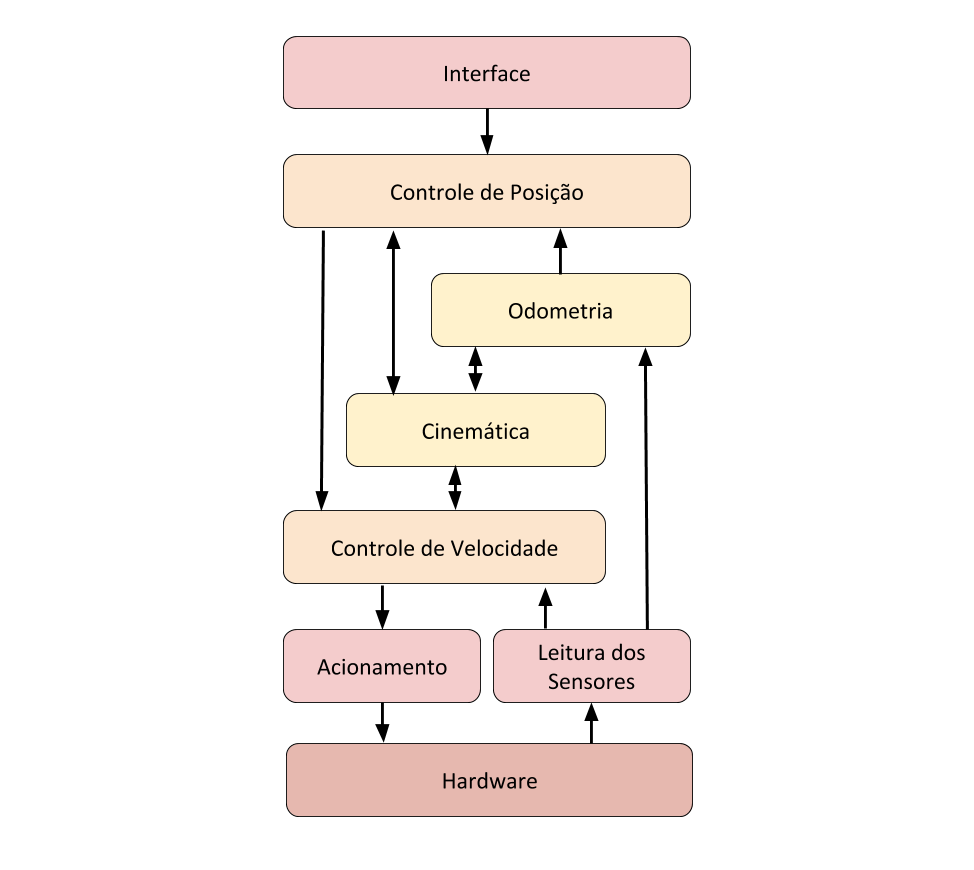
\includegraphics[width = 0.6\textwidth]{imagens/sistema}
  \caption{Estrutura e hierarquia dos subsistemas.}
  \label{fig:sistema}
\end{figure}

Foram omitidos da figura, por simplicidade, os algoritmos de limitação de velocidade, de compensação de zona-morta e de FALTA UM.

O \textit{software} foi implementado em um computador embarcado Raspberry Pi, conforme proposto por \citet{ritter2016modelagem}. O \textbf{Raspberry Pi} é um \emph{single board computer}, que utiliza a arquitetura \acrshort{arm} em seu processador, ideal para dispositivos alimentados por baterias por consumir pouca energia e gerar pouco calor. O processador possui quatro núcleos, e um \emph{clock} de 1,2 GHz -- poder computacional equivalente há um computador de mesa comum. O \acrshort{rpi} utiliza um sistema operacional GNU/Linux, e \emph{software} deve ser desenvolvido para ser executado nesta plataforma. Há ainda 40 pinos de \acrshort{gpio} que podem ser utilizados para conectar sensores, atuadores e diversos componentes, e suporte nativo a \acrshort{i2c} \citep{upton2014raspberry}.

Uma preocupação que se tem ao utilizar um computador se deve ao fato do mesmo não ser caracterizado como um sistema de tempo real. No caso, temporização precisa não é garantida, e a ordem de prioridade de execução de tarefas é gerenciada pelo \textit{kernel VERIFICA}. Assim, funções que seriam executadas imediatamente em um microcontrolador (como rotinas de interrupção), são executadas ``assim que possível'', o que pode prejudicar o desempenho do sistema.

Com isso em mente, foi implementado um software com a linguagem C++, uma das linguagens suportadas pelas bibliotecas de acesso às portas \acrshort{gpio} que apresenta melhores velocidades de execução. \textit{(citar alguém?)} Com esta escolha de linguagem, também se pode utilizar parcialmente os códigos implementados para o trabalho de \citet{ritter2016modelagem}, que também utilizou a mesma linguagem de programação.

%ordem das coisas:
%-análise dos códigos de cinemática
%-desmembramento das funções do ritter

A primeira etapa do desenvolvimento foi a de separar o código desenvolvido por \citet{ritter2016modelagem} em duas partes: uma destinada aos comandos de acionamento, que naquele trabalho eram realizados em um simulador, e outra relacionada à cinemática do robô. Esta segunda porção foi encapsulada em uma biblioteca própria, que pode assim ser utilizada por qualquer desenvolvedor de software no âmbito de TOMR. A biblioteca foi então devidamente analisada e testada no computador embarcado. A biblioteca se chama kinematics.h.

%-código de acionamento dos motores
%-bilbioteca orientada a objetos para o acionamento de cada motor e modularização do código\\
Em seguida, foram realizados testes de acionamento e leitura dos sensores dos motores, se baseando na biblioteca PIGPIO \textit{como referenciar a bibioteca?} \citep{pigpio} para a utilização das entradas e saídas físicas do computador. Utilizando o conceito de orientação a objetos, foi criada uma classe que descreve os parâmetros de cada conjunto motor/sensor e as operações a serem realizadas sobre eles. Esta classe foi batizada de RPiInterface, pois realiza a interface entre o processamento da Raspberry Pi com os sensores e atuadores físicos.

A leitura dos sensores de velocidade, no entanto, foi realizada no main.cpp, devido à utilização de uma biblioteca específica de decodificação de encoders utilizada (rotary\_encoder.h), que implementa interrupções e \textit{n sei direito pq não rolou deixar dentro da classe.}

As equações implementadas relacionam as matrizes de transformação com a velocidade linear da periferia das rodas, $\dot{\phi}_i r$, em m/s. A leitura dos encoders é realizada em pulsos/$\mu$s. O fator de conversão aplicado é (em teoria) 534.18. Ao se utilizar o comando inverseKinematicsWorld, se obtêm as velocidades em m/s e a velocidade angular em rad/s.

% 341.2/2pi pulsos/rad -> 54.3 pulsos/rad (0.01842 rad/pulso, 0.0029308323 rotações/pulso)
% VER O PAPEL NO MURAL

%-controle de velocidade
Na mesma classe se implementou a função de atualização da lei de controle de velocidade de cada motor. Esta função é executada a cada 10ms pela função loop() (mostrada no \hyperref[sec:custo]{Apêndice B})

Se implementou um controle proporcional simples, COLOCAR A LEI AQUI, mas se ontou que em trajetórias que necessitam do movimento das trê rodas em velocidades muito distintas se tem problemas. Para se mover em uma reta no eixo x, por exemplo, apenas as rodas 1 e 3 (verificar numeros) precisam girar, e na mesma velocidade, e fica simples de ver que o desempenho do controlador para as duas rodas vai ser similar. Mais sobre o tema é descrito na próxima seção. No entanto, na movimentação no eixo y são necessárias q a roda 1 esteja girando com o triplo da velocidade das outras duas (verificar), e assim vence a zona morta muito antes. Para solucionar isso, se utilizou uma técnica de eliminação de zona morta, confrome sdkasldkjabsdlkjbladkjbsa.

%implementação dos algoritmos de odometria
Após a verificação do sistema de controle de velocidade, foram implementadas da maneira descrita na seção anterior as fórmulas relacionadas à odometria. Os dados de velocidade foram obtidos se acumulando diretamente a contagem de pulsos de em cada encoder, e avaliando a taxa de variação desta contagem e de uma contagem anterior no intervalo de tempo em que a função foi chamada novamente. A precisão da odometria é essencial para o funcionamento do controle de posição, e portanto o sistema foi testado antes do desenvolvimento do outro, com os resultados descritos na seção seguinte.

%-implementação do controle de posição
O controle de posição foi implementado para ser executado dentro da mesma função loop().

%algoritmo de limitação de velocidade, escalonamento \\
Seguir o perfil de velocidade não é muito fácil, visto que dead zone. budibudibuidi \citet{indiveri2009swedish} trata saturação.

%-organização do código
%-interface com o usuário
Além de utilizar os comandos fornecidos por \citet{ritter2016modelagem}, foram implementados os modos de movimentação citados por \citet{loh2003mechatronics}: translação retilínea , translação curvilínea -- ambas sem alteração na orientação --, rotação pura e um caminho combinado de rotação em torno do seu centro e translação retilínia em relação às referências globais.

%-sequencia final de operação do código
Se notou que o acionamento dos motores depende de a
O procedimento de opereação pode ser representado pelo diagrama apresentado na Figura \ref{fig:operation}.

\begin{figure}[h]
  \centering
  
\includegraphics[width = 0.45\textwidth]{imagens/edc}
  \caption{Fluxograma de operação do robô. TROCAR FIGURA}
  \label{fig:operation}
\end{figure}

Fazer algum arquivo de log para cada execução?

\section{Avaliação experimental}
\label{sec:experimental}

Se deseja avaliar o comportamento dos algoritmos implementados e da modelagem realizada operando o robô em três situações:
\begin{itemize}
  \item{trajetória retilínea, sem nenhum movimento de rotação, em diversas direções e com diversas velocidades de acionamento, conforme mostrado na Figura \ref{fig:reta};}
  \item{trajetória de rotação pura, analisando a variação de ângulo atingida em função do ângulo desejado e da velocidade desejada. Tal situação é ilustrada na Figura \ref{fig:giro};}
  \item{trajetória híbrida, realizando tanto uma translação retilínea arbitrária quanto uma rotação sobreposta, como no diagrama da Figura \ref{fig:hibrida}.}
\end{itemize}

\begin{figure}[h]
  \centering
  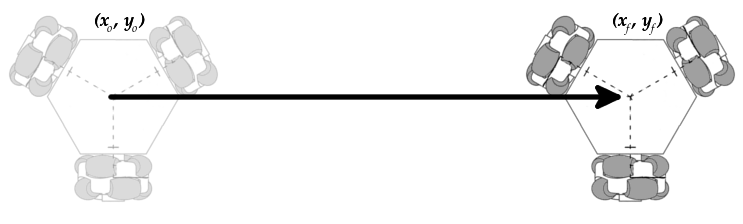
\includegraphics[width = 0.8\textwidth]{imagens/reta}
  \caption{Trajetória retilínea pura.}
  \label{fig:reta}
\end{figure}

\begin{figure}[h]
  \centering
  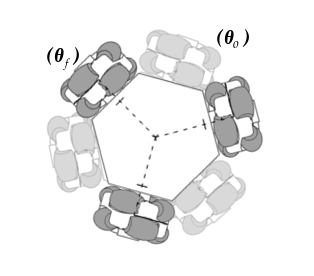
\includegraphics[width = 0.35\textwidth]{imagens/giro}
  \caption{Trajetória de giro.}
  \label{fig:giro}
\end{figure}

\begin{figure}[h]
  \centering
  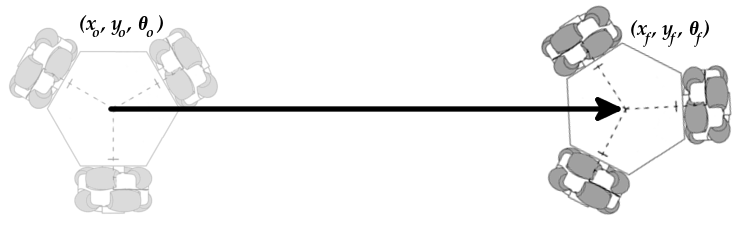
\includegraphics[width = 0.8\textwidth]{imagens/hibrida}
  \caption{Trajetória combinada.}
  \label{fig:hibrida}
\end{figure}

Se espera com a primeira trajetória, avaliar a robustez dos algoritmos quando se necessita o acionamento combinado de múltiplas rodas. Por exemplo, no eixo X, não há necessidade de movimento em uma das rodas. Em outras direções, se introduz movimentos mais lentos das rodas, o que já se viu que é um problema por causa do atrito viscoso da caixa de redução.

Com a trajetória de giro, em que as três rodas devem operar com a mesma velocidade, se deseja avaliar alguma coisa relacionada a isso. Na última trajetória, híbrida, se deseja mostrar o funcionamento do algoritmo de limitação de velocidade, e os efeitos deste fator.

Se notou que o acionamento dos motores depende de alguns fatores. Variando a frequência dos PWMs mudou o q?

O protótipo foi acionado sobre um papel enorme, com duas canetas de cores distintas instaladas nos orifícios destinados a tal.
